% The qLDPC Challenge -- talk slides
% Build: pdflatex qldpc-challenge-slides.tex  (run twice)
\documentclass[11pt,aspectratio=169]{beamer}

\usepackage[T1]{fontenc}
\usepackage{lmodern}
\usepackage{amsmath,amssymb}
\usepackage{booktabs}
\usepackage{tikz}
\usetikzlibrary{positioning,arrows.meta,fit}

% ---------- palette (matches the project site) ----------
\definecolor{ink}{RGB}{24,32,40}
\definecolor{trust}{RGB}{21,110,84}
\definecolor{agent}{RGB}{70,84,156}
\definecolor{flag}{RGB}{179,55,43}
\definecolor{muted}{RGB}{90,100,114}
\definecolor{paper}{RGB}{246,247,244}
\definecolor{trustwash}{RGB}{233,242,236}
\definecolor{agentwash}{RGB}{237,239,248}

% ---------- minimal beamer look ----------
\usetheme{default}
\setbeamertemplate{navigation symbols}{}
\setbeamercolor{structure}{fg=trust}
\setbeamercolor{normal text}{fg=ink,bg=white}
\setbeamercolor{frametitle}{fg=ink,bg=white}
\setbeamerfont{frametitle}{series=\bfseries,size=\large}
\setbeamertemplate{frametitle}{\vspace{10pt}\insertframetitle\par
  \vspace{2pt}{\color{trust}\rule{28pt}{2pt}}\vspace{2pt}}
\setbeamertemplate{footline}{%
  \hfill{\color{muted}\scriptsize\insertframenumber\,/\,\inserttotalframenumber}\hspace{12pt}\vspace{6pt}}
\setbeamertemplate{itemize item}{\color{trust}$\blacktriangleright$}
\setbeamertemplate{itemize subitem}{\color{muted}$\triangleright$}
\setbeamercolor{block title}{bg=trustwash,fg=trust}
\setbeamercolor{block body}{bg=paper,fg=ink}
\setbeamercolor{block title alerted}{bg=flag!12,fg=flag}
\setbeamercolor{block body alerted}{bg=paper,fg=ink}

\newcommand{\GF}{\mathbb{F}_2}
\newcommand{\rank}{\operatorname{rank}}
\newcommand{\wt}{\operatorname{wt}}
\newcommand{\code}[1]{\texttt{\small #1}}

\title{\textbf{The qLDPC Challenge}\\[6pt]
  \large A public, automatically verified leaderboard for quantum LDPC codes}
\author{Unitary Foundation\\[2pt]
  \texttt{github.com/unitaryfoundation/qldpc-challenge}}
\date{}

\begin{document}

\begin{frame}
  \titlepage
\end{frame}

\begin{frame}{This talk}
  \begin{enumerate}\setlength{\itemsep}{10pt}
    \item Why quantum error correction, in five minutes
    \item Quantum LDPC codes: beyond the surface code
    \item Distance: the hard part, and how claims can be checked anyway
    \item The Challenge: an autoresearch loop with a trusted referee
  \end{enumerate}
\end{frame}

% =====================================================================
\section{Quantum error correction}
% =====================================================================

\begin{frame}{Why error correction at all}
  \begin{itemize}\setlength{\itemsep}{8pt}
    \item Physical qubits err at rates $\sim 10^{-3}$--$10^{-2}$ per operation;
          useful algorithms need $10^{-10}$ or better.
    \item Fix: encode $k$ \textbf{logical} qubits redundantly into $n$
          \textbf{physical} qubits, measure carefully chosen parities
          (\emph{syndromes}), and undo errors faster than they accumulate.
    \item \textbf{Threshold theorem}: below a constant physical error rate, logical
          errors can be suppressed exponentially in the code distance $d$.
    \item The whole game is the \textbf{overhead}: how many physical qubits per
          logical qubit, at a given protection level?
  \end{itemize}
\end{frame}

\begin{frame}{Stabilizer codes and the CSS recipe}
  A CSS code is specified by two binary parity-check matrices:
  \[
    H_X \in \GF^{\,r_X \times n}, \qquad
    H_Z \in \GF^{\,r_Z \times n}, \qquad
    \text{with } H_X H_Z^{\mathsf T} = 0 \ (\mathrm{mod}\ 2).
  \]
  \begin{columns}[T]
    \begin{column}{0.55\textwidth}
      \begin{itemize}\setlength{\itemsep}{6pt}
        \item Each row of $H_X$ is an $X$-type parity check (a stabilizer);
              each row of $H_Z$ a $Z$-type one. The orthogonality condition makes
              them all commute.
        \item Number of logical qubits:
              \[ k = n - \rank H_X - \rank H_Z. \]
        \item Everything about the code is \emph{recomputable} from
              $(H_X, H_Z)$ --- a fact the Challenge leans on heavily.
      \end{itemize}
    \end{column}
    \begin{column}{0.4\textwidth}
      \begin{block}{Errors, split in two}
        Bit flips ($X$) are caught by $Z$-checks; phase flips ($Z$) by
        $X$-checks. A CSS code is two classical codes stitched together at the
        commutation condition.
      \end{block}
    \end{column}
  \end{columns}
\end{frame}

\begin{frame}{The benchmark: the surface code}
  \begin{columns}[T]
    \begin{column}{0.55\textwidth}
      \begin{itemize}\setlength{\itemsep}{8pt}
        \item Qubits on a 2D grid; every check touches only its
              \textbf{4 neighbours} $\Rightarrow$ easy to build and measure.
        \item Distance grows with the lattice: $d \sim \sqrt{n}$.
        \item But it encodes \textbf{one} logical qubit per patch:
              \[ k/n \longrightarrow 0. \]
        \item A useful machine needs \emph{thousands} of patches --- millions of
              physical qubits.
      \end{itemize}
      \medskip
      \emph{Can we keep the low-weight checks but get a constant rate?}
    \end{column}
    \begin{column}{0.42\textwidth}
      \centering
      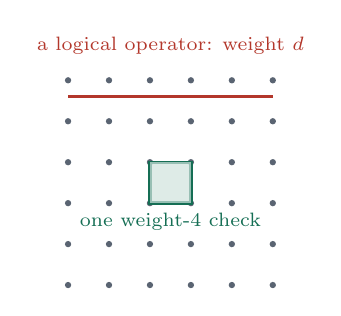
\begin{tikzpicture}[scale=0.52]
        \foreach \i in {0,...,5} \foreach \j in {0,...,5}
          \fill[muted] (\i,\j) circle (2.2pt);
        \draw[trust, very thick] (2,2) -- (3,2) -- (3,3) -- (2,3) -- cycle;
        \fill[trust!20, opacity=0.7] (2,2) rectangle (3,3);
        \node[trust, font=\scriptsize] at (2.5,1.55) {one weight-4 check};
        \draw[flag, very thick] (0,4.6) -- (5,4.6);
        \node[flag, font=\scriptsize] at (2.5,5.85) {a logical operator: weight $d$};
      \end{tikzpicture}
    \end{column}
  \end{columns}
\end{frame}

% =====================================================================
\section{qLDPC codes}
% =====================================================================

\begin{frame}{Quantum LDPC codes}
  \textbf{LDPC} $=$ low-density parity checks: every check touches $O(1)$ qubits
  and every qubit sits in $O(1)$ checks --- the property that makes syndrome
  measurement practical.
  \begin{itemize}\setlength{\itemsep}{8pt}
    \item Breakthrough (2020s): families with \textbf{constant rate and linear
          distance} exist --- asymptotically ``good'' quantum codes.
    \item Practical frontier: small-to-medium block codes that beat the surface
          code's overhead \emph{today}, e.g.\ IBM's bivariate-bicycle
          ``gross code'' $[[144,12,12]]$: 12 logical qubits at distance 12 from
          144 data qubits, weight-6 checks.
    \item Headline figure of merit used throughout the Challenge:
          \[ \text{efficiency} \;=\; \frac{k\,d^2}{n}
             \qquad (\text{surface code} \approx 1,\quad
                     \text{gross code} = 12,\quad
                     \text{board record} = 21.78). \]
  \end{itemize}
\end{frame}

\begin{frame}{Why $kd^2/n$? A yardstick calibrated to two dimensions}
  \begin{block}{Bravyi--Poulin--Terhal bound (2010)}
    Any code whose checks are geometrically local in a 2D layout obeys
    \[ k\,d^2 \;\le\; c\,n \qquad\Longleftrightarrow\qquad \frac{k\,d^2}{n} \le c, \]
    with $c$ a constant depending only on the check range --- not on $n$.
  \end{block}
  \begin{itemize}\setlength{\itemsep}{7pt}
    \item So for \textbf{2D-local codes the metric cannot grow}: the surface code
          ($k=1$, $d\sim\sqrt n$) already \emph{saturates the scaling} at
          $kd^2/n \approx 1$; better 2D-local codes only improve the constant
          (the Challenge's \code{2d-local} tracks live here).
    \item Which is exactly why it makes a good yardstick: $kd^2/n \gg 1$
          \textbf{quantifies how far beyond a strict 2D layout} a code performs.
          The board record of $21.78$ is a statement about connectivity, not
          just cleverness.
  \end{itemize}
\end{frame}

\begin{frame}{Dimensionality raises the ceiling}
  \small
  BPT generalizes to checks local in $D$ dimensions:
  $\;k\,d^{\,2/(D-1)} \le O(n)$ and $d \le O(n^{(D-1)/D})$
  $\;\Rightarrow\; kd^2/n \le O\!\left(n^{\,2(D-2)/D}\right)$.
  \begin{center}
  \renewcommand{\arraystretch}{1.15}
  \begin{tabular}{@{}llll@{}}
    \toprule
    \textbf{Layout} & \textbf{BPT tradeoff} & \textbf{Max $d$} & \textbf{Ceiling on $kd^2/n$} \\
    \midrule
    2D local & $kd^{2} \le O(n)$ & $O(\sqrt{n})$ & $O(1)$ \\
    3D local & $kd \le O(n)$ & $O(n^{2/3})$ & $O(n^{2/3})$ \\
    all-to-all & --- & $\Theta(n)$ & $\Theta(n^{2})$ \\
    \bottomrule
  \end{tabular}
  \end{center}
  \begin{itemize}\setlength{\itemsep}{3pt}
    \item The ceilings are \textbf{achievable}, not just bounds: BPT-saturating
          constructions exist in every $D$ (Portnoy '23; Williamson--Baspin;
          Lin--Wills--Hsieh); ``good'' codes reach $k,d = \Theta(n)$
          (Panteleev--Kalachev '21).
    \item So $kd^2/n$ is a \textbf{constant-vs-growing diagnostic}: flat for
          planar hardware, polynomially higher with every dimension of
          long-range connectivity.
    \item On the leaderboard this needs \textbf{no new metric}: locality class is
          computed from the layout, $kd^2/n$ compared only \emph{within} a
          class --- a \code{3d-local} track would slot in unchanged.
  \end{itemize}
\end{frame}

\begin{frame}{One structure, three generalizations}
  Most board entries are \textbf{two-block} codes:
  \[
    H_X = [\,A \mid B\,], \qquad H_Z = [\,B^{\mathsf T} \mid A^{\mathsf T}\,],
    \qquad AB = BA \;\Rightarrow\; H_X H_Z^{\mathsf T} = 0 .
  \]
  \begin{itemize}\setlength{\itemsep}{7pt}
    \item \textbf{Bivariate bicycle (BB)}: $A, B$ are sparse polynomials in two
          commuting cyclic shifts $x, y$ on a torus $\mathbb{Z}_\ell \times \mathbb{Z}_m$
          --- commutativity is free.
    \item \textbf{2BGA}: replace the torus by \emph{any} finite group $G$; $A$
          acts by left multiplication, $B$ by right multiplication, which always
          commute. Non-abelian $G$ (dihedral, metacyclic) reaches parameters BB
          cannot, including odd $k$.
    \item \textbf{Coset codes}: qubits on cosets $G/H$ --- the current
          record-efficiency family ($k d^2/n = 21.78$ at $[[180,20,14]]$).
  \end{itemize}
  \medskip
  Separate track: \textbf{2D-local planar} codes with open boundaries ---
  qLDPC codes you could lay out on a chip bilayer, checks within radius
  $\sim 3$ on the grid.
\end{frame}

% =====================================================================
\section{Distance}
% =====================================================================

\begin{frame}{Distance: what it is}
  A \textbf{logical operator} acts on the encoded qubits without triggering any
  check:
  \[
    d_X \;=\; \min\Bigl\{\, \wt(v) \;:\; H_Z v = 0,\;\;
      v \notin \operatorname{rowspace}(H_X) \,\Bigr\},
    \qquad d = \min(d_X, d_Z).
  \]
  \begin{itemize}\setlength{\itemsep}{8pt}
    \item In the kernel: commutes with every $Z$-check.
          Outside the rowspace: not itself a product of stabilizers.
    \item $d$ is the weight of the \emph{cheapest undetectable error} ---
          it sets the protection level, and it enters the figure of merit
          \emph{squared}.
    \item \alert{Computing $d$ exactly is NP-hard.} Every distance number you
          read in a paper was produced by a bounded search --- and bounded
          searches miss things.
  \end{itemize}
\end{frame}

\begin{frame}{Measuring distance in practice}
  \begin{columns}[T]
    \begin{column}{0.5\textwidth}
      \textbf{Upper bounds: find \emph{a} logical}
      \begin{itemize}\setlength{\itemsep}{6pt}
        \item \emph{Randomized information-set search}: RREF the kernel basis
              under random column orders; light rows (and their pairwise sums)
              are candidate logicals.
        \item \emph{Decoder residuals}: inject errors, decode with BP+OSD;
              a decoding failure that commutes with all checks \emph{is} a
              logical operator.
        \item Either way the output is an explicit \textbf{witness}: a vector
              anyone can check in milliseconds. It proves $d \le \wt(v)$ ---
              trustlessly.
      \end{itemize}
    \end{column}
    \begin{column}{0.48\textwidth}
      \textbf{Exact values: prove nothing lighter exists}
      \begin{itemize}\setlength{\itemsep}{6pt}
        \item Integer program per logical class: minimize $\wt(v)$ subject to
              $H_Z v = 0 \pmod 2$ and $\ell \cdot v = 1 \pmod 2$.
        \item Feasible for small / low-rate codes; hopeless for large high-rate
              ones.
      \end{itemize}
      \begin{alertblock}{The trap}
        A \emph{high} estimate from a \emph{short} search looks like a great
        code. It usually means the search hasn't found the light logical yet.
        Distance claims need adversarial checking.
      \end{alertblock}
    \end{column}
  \end{columns}
\end{frame}

% =====================================================================
\section{The Challenge}
% =====================================================================

\begin{frame}{What the Challenge is}
  \begin{itemize}\setlength{\itemsep}{8pt}
    \item A \textbf{public leaderboard} of qLDPC codes: one JSON file per code,
          in a git repository, with a static site on top.
          \hfill {\color{muted}\small 41 codes today}
    \item Every claim is \textbf{recomputed from the parity checks} --- $n$, $k$,
          CSS commutation, check weights, distance witnesses, 2D-locality radius.
          Nothing is trusted from the submitter.
    \item Codes compete on \textbf{Pareto frontiers} inside track cells
          (check-weight class $\times$ locality class), never on a single score.
    \item Designed so that \textbf{LLM research agents} can do the searching ---
          with a referee they cannot talk their way past.
  \end{itemize}
\end{frame}

\begin{frame}{Three zones, one direction of trust}
  \centering
  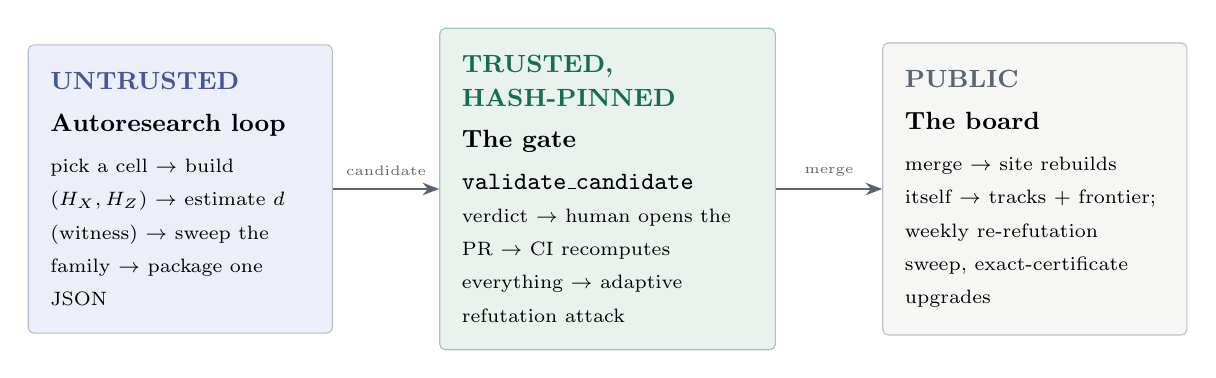
\begin{tikzpicture}[
      zone/.style={rounded corners=2pt, minimum height=2.35cm, inner sep=8pt},
      lbl/.style={font=\bfseries\small, anchor=north west},
      item/.style={font=\scriptsize, anchor=north west, text width=3.35cm},
      arr/.style={-{Stealth[length=6pt]}, thick, muted}]
    \node[zone, fill=agentwash, draw=agent!40] (a) at (0,0)
      {\begin{minipage}{3.3cm}\raggedright\vspace{2pt}
        {\color{agent}\bfseries\small UNTRUSTED}\\[3pt]
        {\bfseries\small Autoresearch loop}\\[3pt]
        {\scriptsize pick a cell $\to$ build $(H_X,H_Z)$ $\to$
         estimate $d$ (witness) $\to$ sweep the family $\to$
         package one JSON}\vspace{2pt}\end{minipage}};
    \node[zone, fill=trustwash, draw=trust!40, right=1.35cm of a] (b)
      {\begin{minipage}{3.7cm}\raggedright\vspace{2pt}
        {\color{trust}\bfseries\small TRUSTED, HASH-PINNED}\\[3pt]
        {\bfseries\small The gate}\\[3pt]
        {\scriptsize \code{validate\_candidate} verdict $\to$ human opens the PR
         $\to$ CI recomputes everything $\to$ adaptive refutation attack}
        \vspace{2pt}\end{minipage}};
    \node[zone, fill=paper, draw=muted!40, right=1.35cm of b] (c)
      {\begin{minipage}{3.3cm}\raggedright\vspace{2pt}
        {\color{muted}\bfseries\small PUBLIC}\\[3pt]
        {\bfseries\small The board}\\[3pt]
        {\scriptsize merge $\to$ site rebuilds itself $\to$ tracks + frontier;
         weekly re-refutation sweep, exact-certificate upgrades}
        \vspace{2pt}\end{minipage}};
    \draw[arr] (a) -- node[above=1pt, font=\tiny, muted] {candidate} (b);
    \draw[arr] (b) -- node[above=1pt, font=\tiny, muted] {merge} (c);
  \end{tikzpicture}

  \vspace{6pt}
  \begin{block}{The one rule (from the agent manual, \code{AUTORESEARCH.md})}
    No code is a find until \code{validate\_candidate} returns
    \code{passed:\,true}. You may write and run any code you like --- but you do
    not get to decide whether a code is good.
  \end{block}
\end{frame}

\begin{frame}{The CI gauntlet, per submission}
  \small
  \begin{enumerate}\setlength{\itemsep}{5pt}
    \item \textbf{Scope}: a PR adding a code may not touch workflows, the schema,
          or \code{verify/} --- a submission cannot change its own judge.
          One new code per PR.
    \item \textbf{Integrity pin}: SHA-256 of the whole trusted stack against a
          committed manifest; any drift fails the build.
    \item \textbf{Self-tests}: the verifier must still \emph{reject} known-bad
          submissions and known over-claims.
    \item \textbf{Recomputation}: $n$, $k$, CSS, weights, witnesses, locality ---
          recomputed by the \emph{base branch's} verifier.
    \item \textbf{Adaptive refutation}: two independent searches attack the
          distance claim. Budget scales with size ($2500 + 40n$ trials);
          a claim that advances a frontier pays
          $3 \text{ seeds} \times (25000 + 120n)$ trials before it earns the
          record. One lighter logical found $\Rightarrow$ PR fails, witness
          printed.
    \item \textbf{Authorship}: the PR author must be a listed author of the code.
  \end{enumerate}
\end{frame}

\begin{frame}{Geometry is verified too: you cannot lie about locality}
  The 2D-local tracks matter (they carry the $kd^2/n \le c$ ceiling), so class
  membership is \textbf{computed, never declared}: a submission carries its
  layout --- coordinates plus a layer count --- as a \emph{checkable
  certificate}, exactly like the distance witness.
  \begin{columns}[T]
    \begin{column}{0.56\textwidth}
      \begin{itemize}\setlength{\itemsep}{5pt}
        \item a coordinate for \textbf{every} qubit;
        \item \textbf{no cramming}: at most \code{layers} qubits per site,
              distinct sites $\ge 1$ apart --- a small radius cannot be faked by
              collapsing or rescaling points;
        \item the interaction radius is \textbf{measured} (largest check
              diameter) and must sit under the class cap;
        \item a dishonest or missing layout is not rejected --- the code simply
              competes as \code{unrestricted}, the harder cell.
      \end{itemize}
    \end{column}
    \begin{column}{0.42\textwidth}
      \centering
      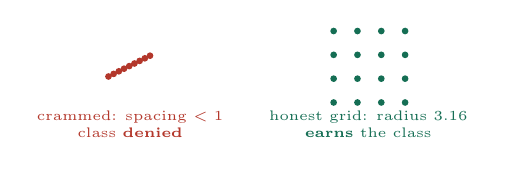
\begin{tikzpicture}[scale=0.55]
        % crammed layout: denied
        \foreach \i in {0,...,8} \fill[flag] (0.12*\i, 0.35+0.06*\i) circle (2.2pt);
        \node[flag, font=\tiny, align=center] at (0.5,-0.75)
          {crammed: spacing $<1$\\class \textbf{denied}};
        % honest grid: earned
        \foreach \i in {0,...,3} \foreach \j in {0,...,3}
          \fill[trust] (5.2+0.55*\i, 0.55*\j-0.25) circle (2.2pt);
        \node[trust, font=\tiny, align=center] at (6.0,-0.75)
          {honest grid: radius 3.16\\\textbf{earns} the class};
      \end{tikzpicture}
      \par\vspace{6pt}
      {\scriptsize\color{muted} Field test: retro-tagging seven planar codes,
      the first (wrong) embedding measured radius 10.2, growing with size ---
      refused. The correct one measured 3.16, size-independent --- earned.}
    \end{column}
  \end{columns}
\end{frame}

\begin{frame}{Distance claims are tiered by how they were earned}
  \centering
  \renewcommand{\arraystretch}{1.5}
  \begin{tabular}{@{}lll@{}}
    \toprule
    \textbf{Tier} & \textbf{Meaning} & \textbf{Earned by} \\
    \midrule
    {\color{ink}$d \le v$} & upper bound & witness checked trustlessly, milliseconds \\
    {\color{trust}$d = v$} & exact & server MILP certificate committed to \code{certs/} \\
    {\color{flag}refuted} & claim killed & any search finding a lighter logical, witness attached \\
    \bottomrule
  \end{tabular}

  \vspace{12pt}
  \begin{itemize}
    \item 27 of 41 board codes hold an exact certificate.
    \item The other defense is time: a \textbf{weekly random-seed sweep}
          re-attacks every entry on the board, forever.
  \end{itemize}
\end{frame}

\begin{frame}{Case study: the pipeline correcting an over-claim}
  \textbf{$[[294,8,19]]$, a 2BGA code on a metacyclic group} (June 2026)
  \begin{enumerate}\setlength{\itemsep}{8pt}
    \item An LLM agent sweeping metacyclic 2BGA codes surfaced a candidate
          claiming $d = 20$ (with a $Z$-side claim of 25). It \emph{passed} the
          standard 8k-trial gate.
    \item Deep refutation --- 60k trials across independent seeds --- found a
          \textbf{weight-19 $Z$-logical}: the claim was an artifact of an
          under-converged upper bound.
    \item Resubmitted with the honest $d = 19$ \emph{and the found witness
          attached}; the $X$-side value corroborated by every deep seed.
    \item Merged as a non-dominated weight-8 entry --- and the incident sized
          the adaptive deep gate that now guards every frontier claim.
  \end{enumerate}
  \medskip
  {\color{muted}\small The system's job is not to prevent optimistic claims ---
  it is to make sure they don't survive.}
\end{frame}

\begin{frame}{What it is for}
  \begin{itemize}\setlength{\itemsep}{9pt}
    \item A \textbf{shared, machine-checked record} of which qLDPC codes are best
          under which constraints --- parameters today live scattered across
          papers, hard to reproduce or compare.
    \item A \textbf{benchmark for AI research agents}: the starter kit
          (\code{research/}) is tool-agnostic, pure numpy, and sits on the
          verifier's own linear algebra; \code{AUTORESEARCH.md} is an operating
          manual any model can be pointed at.
    \item A template for \textbf{verification-first open science}: untrusted
          exploration, a pinned referee, and claims that decay gracefully
          (refuted with evidence) instead of persisting as folklore.
  \end{itemize}
  \vspace{8pt}
  \begin{center}
    \structure{\textbf{Beat the frontier:}}\quad
    \texttt{github.com/unitaryfoundation/qldpc-challenge}
  \end{center}
\end{frame}

\begin{frame}[plain]
  \vfill
  \centering
  {\LARGE\bfseries Thanks!}\\[14pt]
  {\color{muted}Live board, starter kit, and the full verification stack:}\\[6pt]
  \texttt{github.com/unitaryfoundation/qldpc-challenge}\\[2pt]
  {\color{muted}\texttt{unitaryfoundation.github.io/qldpc-challenge}}
  \vfill
\end{frame}

\end{document}
